%Matteo Kumar - Leonhard Schatt
% Fortgeschrittenes Physikalisches Praktikum

% Teilauswertung Eichgitter

\section{Vermessung eines Eichgitters}
\subsection{x-y-Verschiebung}
Zuerst soll das Eichgitter vermessen und die Messergebnisse mit den Herstellerangaben verglichen werden. Dazu wird die Aufnahme des AFM mit 
Gwyddion \footnotemark \footnotetext{\url{http://gwyddion.net/}} geöffnet und untersucht.\\
Zur Bestimmung der x-y-Verschiebung werden Strecken über mehrere Raster hinweg und einzelne Raster wie in Abb. \ref{bild:EichWo} gezeigt 
gemessen. 

\begin{figure}[h]
    \centering
    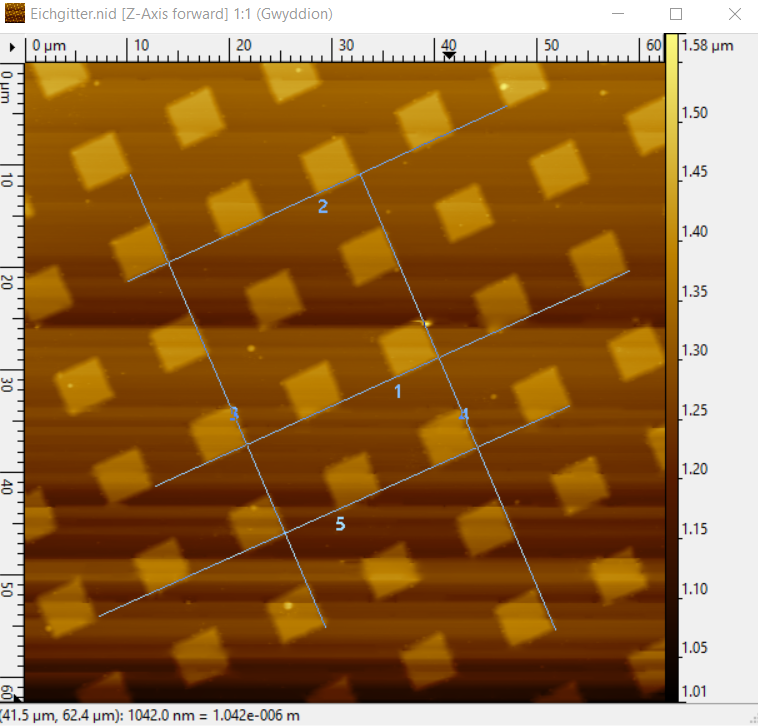
\includegraphics[scale = 0.5]{Bilder/EichGeraden.png}
    \caption{Lage der vermessenen Geraden im Eichgitter}
    \label{bild:EichWo}
\end{figure}
\newpage

Die Längen der Strecken sind:

\begin{center}
    \centering
    \begin{tabular}{l|r r}
        Nummer & Strecke / $\mu m$ & Anzahl Raster \\
        \hline
        1 & 50.9 & 10\\
        2 & 40.8 & 8\\
        3 & 48.2 & 10 \\
        4 & 48.4 & 10 \\
        5 & 50.3 & 10\\
        
    \end{tabular}
\end{center}

Aus den Längen lässt sich der Mittelwert für eine x-y-Versetzung berechnen.

\begin{equation*}
    d_{xy} = 9.942 \mu m
\end{equation*}

Der Hauptfehler dürfte beim Wählen der Start- und Endpunkte 
der zu vermessenden Strecke liegen, da diese nicht sehr gut exakt zu setzen waren. Mithilfe des Vermessungstools wird dieser Fehler auf 
2$\mu m$ pro Strecke abgeschätzt. Nach Fehlerfortpflanzung ergibt sich also:
\begin{equation*}
    s = \sqrt{5}\frac{2 \mu m}{24} = 0.186 \mu m
\end{equation*}

Mit dem internen Fehler des Mikroskops von 1.2\%, ergibt sich für die Versetzung ein Fehler von
\begin{equation*}
    s_d = \sqrt{0.186^2 + (0.012 \cdot 9.942)^2}\, \mu m = 0.22\, \mu m
\end{equation*}

\begin{equation*}
    \textcolor{red}{d_{xy} = (9.94 \pm 0.22) \mu m}
\end{equation*}

Nach Angaben des Herstellers beträgt die Versetzung 10.0 $\mu m$ (s. Protokoll). 
Dieser Wert liegt innerhalb des Fehlers, deshalb kann er als bestätigt angesehen werden. Auffällig ist allerdings, dass sich, 
wenn man die Versetzungen für 'horizontale' (1,2,5) und 'vertikale' (3,4) Strecken getrennt berechnet, unterschiedliche Werte ergeben: 
\begin{equation*}
    d_{xy,h} = 10.14 \mu m, \qquad d_{xy,v} = 9.66 \mu m
\end{equation*}

Dies kann nicht nur Folge von Ungenauigkeiten beim Wählen von den Endpunkten der Strecke sein, dafür ist der berechnete Fehler zu gering. 
Möglich wäre auch noch eine Verkippung des Gitters, sodass die ausgemessenen x-y-Koordinaten nicht exakt der Strecke auf dem Gitter 
entsprechen. In der Tat ist im Profil des Bildes des Eichgitters ein linearer Trend zu erkennen (Abb. \ref{bild:EichKippung}). 
Da die Ergebnisse dennoch gut mit der Theorie übereinstimmen wird an dieser Stelle auf eine Bereinigung verzichtet.

\begin{figure}[h]
    \centering
    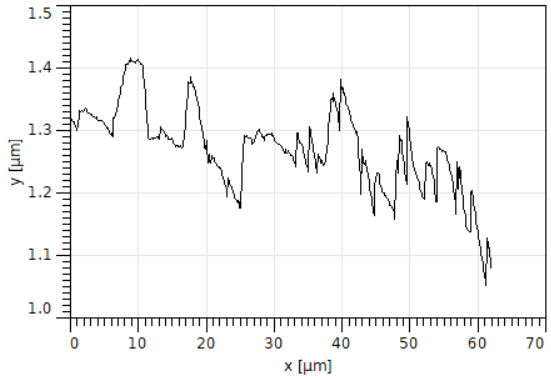
\includegraphics[scale = 0.65]{Bilder/EichKippung.png}
    \caption{Profil des Eichgitters. Ein linearer Trend ist gut zu erkennen - das Gitter ist leicht verkippt.}
    \label{bild:EichKippung}
\end{figure}

\newpage
\subsection{Höhe des Gitters}

Zur Bestimmung der Höhe der Raster wurde ein Höhenprofil von zwei Strecken (s. Abb. \ref{bild:zUebersicht}) erstellt und die Erhöhungen 
vermessen. Die Höhenprofile finden sich in den Abb. \ref{bild:zReihe1} und \ref{bild:zReihe2}. 

\begin{figure}[h]
    \centering
    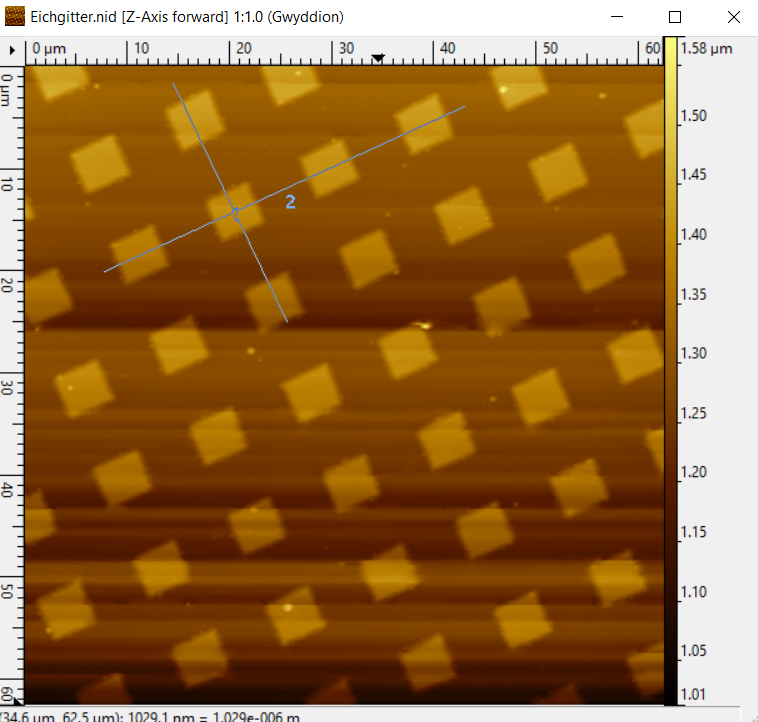
\includegraphics[scale = 0.4]{Bilder/zUebersicht.png}
    \caption{Lage der Geraden zu den Höhenprofilen im Eichgitter}
    \label{bild:zUebersicht}
\end{figure}

\begin{figure}[h]
    \centering
    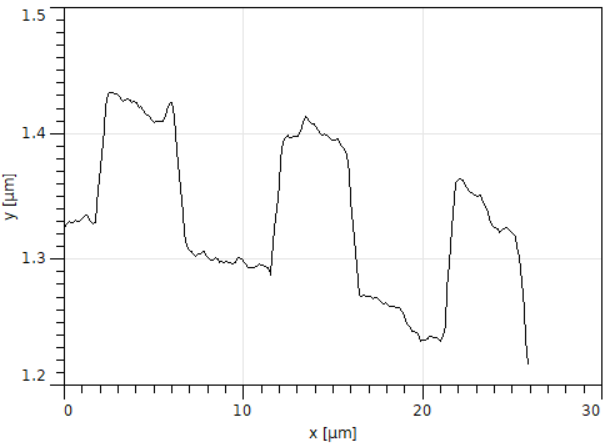
\includegraphics[scale = 0.65]{Bilder/zReihe1.png}
    \caption{Höhenprofil der ersten Geraden}
    \label{bild:zReihe1}
\end{figure}

\begin{figure}[h]
    \centering
    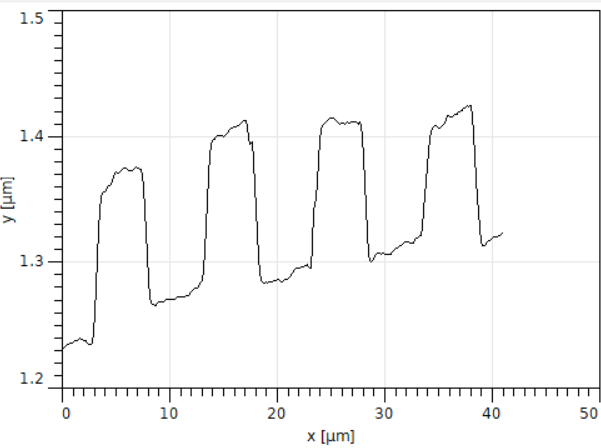
\includegraphics[scale = 0.65]{Bilder/zReihe2.png}
    \caption{Höhenprofil der zweiten Geraden}
    \label{bild:zReihe2}
\end{figure}

\clearpage

Die Höhe der Erhebungen sind: 

\begin{center}
    \centering
    \begin{tabular}{l|r}
        Strecke Reihe 1 /  nm & Strecke Reihe 2 / nm \\
        \hline
        118.0 & 109.6 \\
        107.1 & 119.4 \\
        117.6 & 115.2 \\
        122.3 & 123.7 \\
        119.2 & 128.3 \\
        110.6 & \\
        91.0 & \\
        110.7 & \\
        
    \end{tabular}
\end{center}

Der Mittelwert daraus beträgt $h = 114.823 nm$.
Der Fehler wird hauptsächlich durch die Präzession beim Auswählen der Punkte für die Höhenmessung bestimmt; es war nicht immer klar, 
wo der Anstieg beginnt und endet. Es sei deshalb pro Messung ein Fehler von 5nm angenommen. Über Fehlerfortpflanzung ergibt sich für 
den Fehler des Mittelwerts: 
\begin{equation*}
    s_h = \frac{5}{\sqrt{13}} nm = 1.39 nm
\end{equation*}

Damit ist die Höhe der Erhebungen: 
\begin{equation*}
    \textcolor{red}{h = (114.8 \pm 1.4)nm}
\end{equation*}

Laut Hersteller sollte die Höhe aber 119.0 nm betragen, was außerhalb des Fehlerbereichs liegt (s. Protokoll). Eine Erklärung wäre, dass der Fehler 
zu niedrig abgeschätzt wurde. Wahrscheinlicher ist es aber, dass die Erhöhungen im Laufe der Zeit durch das Vermessen im Contact-Mode 
abgeschliffen wurden. Dafür sprechen auch die an den Helligkeitsunterschieden vor allem in der unteren Hälfte von 
Abb. \ref{bild:zUebersicht} erkennbaren horizontalen Linien über den gesamten Gitterausschnitt. Dies könnten Messfehler des 
AFM sein. Deshalb war auch die Wahl der Strecken für diese Messung nicht ganz einfach, da 
eine Stelle mit möglichst wenig Abnutzung gefunden werden musste. Zum Vergleich ist in Abb. \ref{bild:zUngeeignet} ein dafür 
ungeeignetes Profil zu sehen.

\begin{figure}[h]
    \centering
    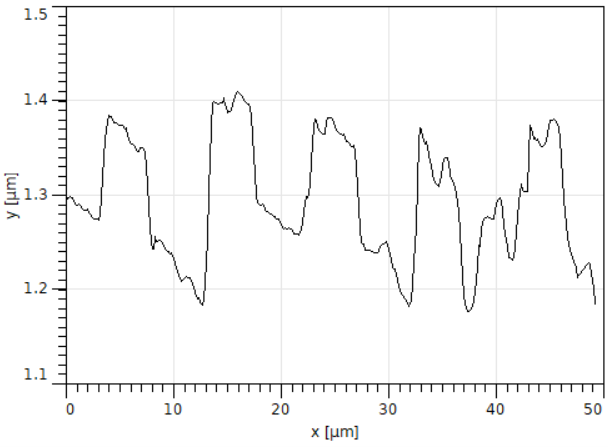
\includegraphics[scale = 0.65]{Bilder/zUngeeignet.png}
    \caption{Ungeeignetes Höhenprofil einer Geraden aus dem Ausschnitt des Eichgitters}
    \label{bild:zUngeeignet}
\end{figure}

\newpage